%%%%%%%%%%%%%%%%%%%%%%%%%%%%%%%%%%%%%%%%%%%%%%%%%%%%%%%%%%%%%%%%
%
%  Template for creating scribe notes for cs229t. borrowed from Rob Schapire 
%
%  Fill in your name, lecture number, lecture date and body
%  of scribe notes as indicated below.
%
%%%%%%%%%%%%%%%%%%%%%%%%%%%%%%%%%%%%%%%%%%%%%%%%%%%%%%%%%%%%%%%%


\documentclass[11pt]{article}

\setlength{\topmargin}{0pt}
\setlength{\textheight}{9in}
\setlength{\headheight}{0pt}
\setlength{\headsep}{0pt}
\setlength{\oddsidemargin}{0.25in}
\setlength{\textwidth}{6in}
\setlength{\parskip}{7pt}
\setlength\parindent{0pt}

\usepackage{latexsym}
\usepackage{amsmath}
\usepackage{amssymb}
\usepackage{amsthm}
\usepackage{epsfig}
\usepackage{url}
\usepackage{mdframed}

\newtheorem{theorem}{Theorem}
\newtheorem{corollary}[theorem]{Corollary}
\newtheorem{lemma}[theorem]{Lemma}
\newtheorem{observation}[theorem]{Observation}
\newtheorem{proposition}[theorem]{Proposition}
\newtheorem{definition}[theorem]{Definition}
\newtheorem{claim}[theorem]{Claim}
\newtheorem{fact}[theorem]{Fact}
\newtheorem{assumption}[theorem]{Assumption}
\newtheorem{remark}[theorem]{Remark}

\newcommand{\E}{\mathbb{E}}
\newcommand{\R}{\mathbb{R}}
\newcommand{\Z}{\mathbb{Z}}
\newcommand{\Prob}{\text{Pr}}
\newcommand{\Var}{\text{Var}}
\newcommand{\Cov}{\text{Cov}}
\newcommand{\norm}[1]{\| #1 \|}
\renewcommand{\epsilon}{\varepsilon}



\newcommand{\draftnotice}{\vbox to 0.25in{\noindent
   \raisebox{0.6in}[0in][0in]{\makebox[\textwidth][r]{\it
    DRAFT --- a final version will be posted shortly}}}
   \vspace{-.25in}\vspace{-\baselineskip}
}

\pagestyle{plain}

\begin{document}

\thispagestyle{empty}

% \draftnotice

\begin{center}
\bf\large CS229T/STATS231: Statistical Learning Theory
\end{center}

\noindent
Lecturer: Tengyu Ma   %%% FILL IN LECTURER (if not RS)
\hfill
Lecture \#4               %%% FILL IN LECTURE NUMBER HERE
\\
Scribe: Weiyun Ma                 %%% FILL IN YOUR NAME HERE
\hfill
October 3, 2018           %%% FILL IN LECTURE DATE HERE

\noindent
\rule{\textwidth}{1pt}

\medskip

%%%%%%%%%%%%%%%%%%%%%%%%%%%%%%%%%%%%%%%%%%%%%%%%%%%%%%%%%%%%%%%%
%% BODY OF SCRIBE NOTES GOES HERE
%%%%%%%%%%%%%%%%%%%%%%%%%%%%%%%%%%%%%%%%%%%%%%%%%%%%%%%%%%%%%%%%

\section{Review and Overview}
%
%\begin{enumerate}
%	\item If appropriate, one paragraph to briefly review the connection to previous lectures.
%	\item An overview paragraph that summarizes the main idea of the lecture at a high-level.
%\end{enumerate}  
%%%
Last time, we introduced the notion of uniform convergence and showed that it holds for finite hypothesis classes. Specifically, we proved that if $\mathcal H$ is a finite hypothesis class with $0 \le l((x,y), h) \le 1$, then with probability at least $1 - \delta$, we have
\begin{equation} \label{UCF}
\forall h\in \mathcal H, |\hat L(h) - L(h)|\le \sqrt{\frac{\log|\mathcal H| + \log \frac{2}{\delta}}{2n}}.\end{equation}
In other words, with probability at least $1-\delta$, for $\emph{every}$ hypothesis in $\mathcal H$, the difference between its training loss and expected loss is upper bounded by a function that depends on $\delta$, the size of the hypothesis space, and the number of training examples.

Unfortunately, the result above does not generalize to the case when the hypothesis class $\mathcal H$ is parameterized by a continuous space, since we can no longer apply union bound over the infinitely many hypotheses in $\mathcal H$. However, as we will see in the first part of this lecture, if the continuous parameter space that defines $\mathcal H$ is bounded, then we can still achieve a result similar to (\ref{UCF}) using a technique called \emph{discretization}.

In the second part of this lecture, we will shift our focus to proving Hoeffding's inequality, which we used last time. Along the way, we will also introduce a few other useful concentration inequalities.

\section{Uniform Convergence for Parameterized Hypothesis Classes}

In this section, we will prove a uniform convergence result similar to (\ref{UCF}) for parameterized hypothesis classes whose parameter spaces are bounded. The high level idea is that we can select a finite subset of representatives from the entire parameter space, and obtain a uniform convergence bound on those representatives by applying Theorem 2 from last lecture. We then show that every other point in the parameter space is close enough to at least one representative, so that uniform convergence can be extended to all points in the parameter space. We call this technique \emph{discretization} of the parameter space.

\subsection{Setup}
Before we formally demonstrate what discretization is, let us first set up a few notations.

Let $\mathcal H$ be a family of hypothesis functions indexed by parameter $\theta$ from some subset $S$ of $\R^p$. Formally, we write $$\mathcal H = \{h_\theta: \theta \in S\subseteq \R^p \}.$$ In this section, we focus on the case $$S = \{\theta \in \R^p: \|\theta\|_2 \le B\},$$ where $B>0$ is fixed. In other words, we constrain our parameter space $S$ to contain only $p$-dimensional vectors whose $\ell_2$ norms are no greater than some positive threshold $B$. 

Recall that in the parameterized setting, we can write the loss function as $l((x, y), h_\theta) = l((x, y), \theta)$. 

The expected loss is defined as $L(\theta) = \E_{(x, y) \sim P}[l((x, y), \theta)],$ where $P$ is a data distribution that is not necessarily the same as the ground truth distribution.

The training loss (or empirical risk) is defined as $\hat L(\theta) = \frac{1}{n}\sum_{i = 1}^{n}[l((x^{(i)}, y^{(i)}), \theta)],$ where $(x^{(1)}, y^{(1)}), \ldots, (x^{(n)}, y^{(n)})$ are $n$ training examples drawn i.i.d. from $P$. 

\subsection{The Uniform Convergence Theorem}
We now state the uniform convergence theorem for our parameterized hypothesis class $\mathcal H$.

\begin{theorem}\label{main}
Suppose $\ell((x,y), \theta) \in [-M,M]$, and $L(\theta), \hat L(\theta)$ are $L$-Lipschitz with respect to the $\ell_2$-norm. Then with probability $\ge 1-O(p^{-10})$, we have
\begin{equation}
    \forall \theta, |\hat L(\theta)- L(\theta)| \lesssim M \sqrt{\frac{p \log(LBn)}{n}}.
\end{equation}
\end{theorem}
Here, we give the definition of \emph{$L$-Lipschitz functions}:
\begin{definition}
Let $L \ge 0$ and $\norm{\cdot}$ be a norm on the domain $D$. A function $L:D \to \R$ is said to be \emph{$L$-Lipschitz} with respect to $\norm{\cdot}$ if for all $\theta, \theta' \in D$, we have
$$
    |L(\theta)-L(\theta')| \le L \norm{\theta-\theta'}.
$$
\end{definition}

We make a few remarks on Theorem \ref{main}:
\begin{remark} \label{Tight}
    The result is not tight. In particular, with a more careful derivation, one can improve the failure probability $O(p^{-10})$ to $O(e^{-p})$.
\end{remark}   

\begin{remark}
    By Theorem \ref{main} and a result (Theorem 2) from last lecture, we have \begin{equation}\label{gen}L(\hat \theta) - L(\theta^*) \lesssim M \sqrt{\frac{p \log (LBn)}{n}}\end{equation} with probability $\ge 1-O(p^{-10})$, where $\theta^* = \underset{\theta \in S}{\mathrm{argmin}}$ $L(\theta)$ is the minimizer of the expected loss over the parameter space. 

    On the other hand, we showed last week that in the asymptotic regime, we have 
    \begin{equation}\label{genAsym}L(\hat \theta) - L(\theta^*) \approx \frac{p}{2n} + o\left(\frac{1}{n}\right) \quad \text{as } n \to \infty,\end{equation}
    where $\theta^*$ is the ground truth parameter. 
    
    Comparing the generalization bound (\ref{gen}) with (\ref{genAsym}), we see that although the rate in (\ref{gen}) has a worse dependency on $n$, (\ref{gen}) does not contrain how large $n$ has to be. Moreover, (\ref{genAsym}) requires well-specification, i.e. it assumes that the data is from the ground truth distribution, while (\ref{gen}) and Theorem \ref{main} do not need any assumption on the data distribution.
\end{remark}

\subsubsection{Discretization of the Parameter Space by $\epsilon$-Covers}
To prove Theorem \ref{main}, we need a measure to discretize the parameter space. We start by defining an \emph{$\epsilon$-cover}:

\begin{definition}
Let $S$ be a set with metric $\rho$, and let $\epsilon>0$. An \emph{$\epsilon$-cover} of $S$ with respect to $\rho$ is a subset $C \subseteq S$ such that $\forall x \in S$, $\exists x' \in C$ such that $\rho(x,x') \le \epsilon$, or equivalently,
$$ S \subseteq \bigcup_{x \in C} \mathrm{Ball}(x, \epsilon, \rho). $$
\end{definition}

The following lemma tells us that our parameter space $S = \{\theta \in \R^p: \|\theta\|_2 \le B\}$ has an $\epsilon$-cover with not too many elements:

\begin{lemma}\label{ECSize}
Let $B,\epsilon>0$ and $S = \{x \in \R^p: \|x\|_2 \le B\}.$ Then there exists an $\epsilon$-cover of $S$ with respect to the $\ell_2$-norm with at most $\left(\frac{3B\sqrt{p}}{\epsilon}\right)^p$ elements.
\end{lemma}


\begin{proof}
We set
$$C = \{ x \in S: x_i = k_i \tfrac{\epsilon}{\sqrt{p}}, k_i \in \Z, |k_i| \le \tfrac{B\sqrt{p}}{\epsilon}  \},  $$
i.e. $C$ is the set of grid points of the grid in $\R^p$ of width $\tfrac{\epsilon}{\sqrt{p}}$ that are contained in $S$. See Figure 1 for an illustration. 
\begin{figure}[h] \label{ECover}
$$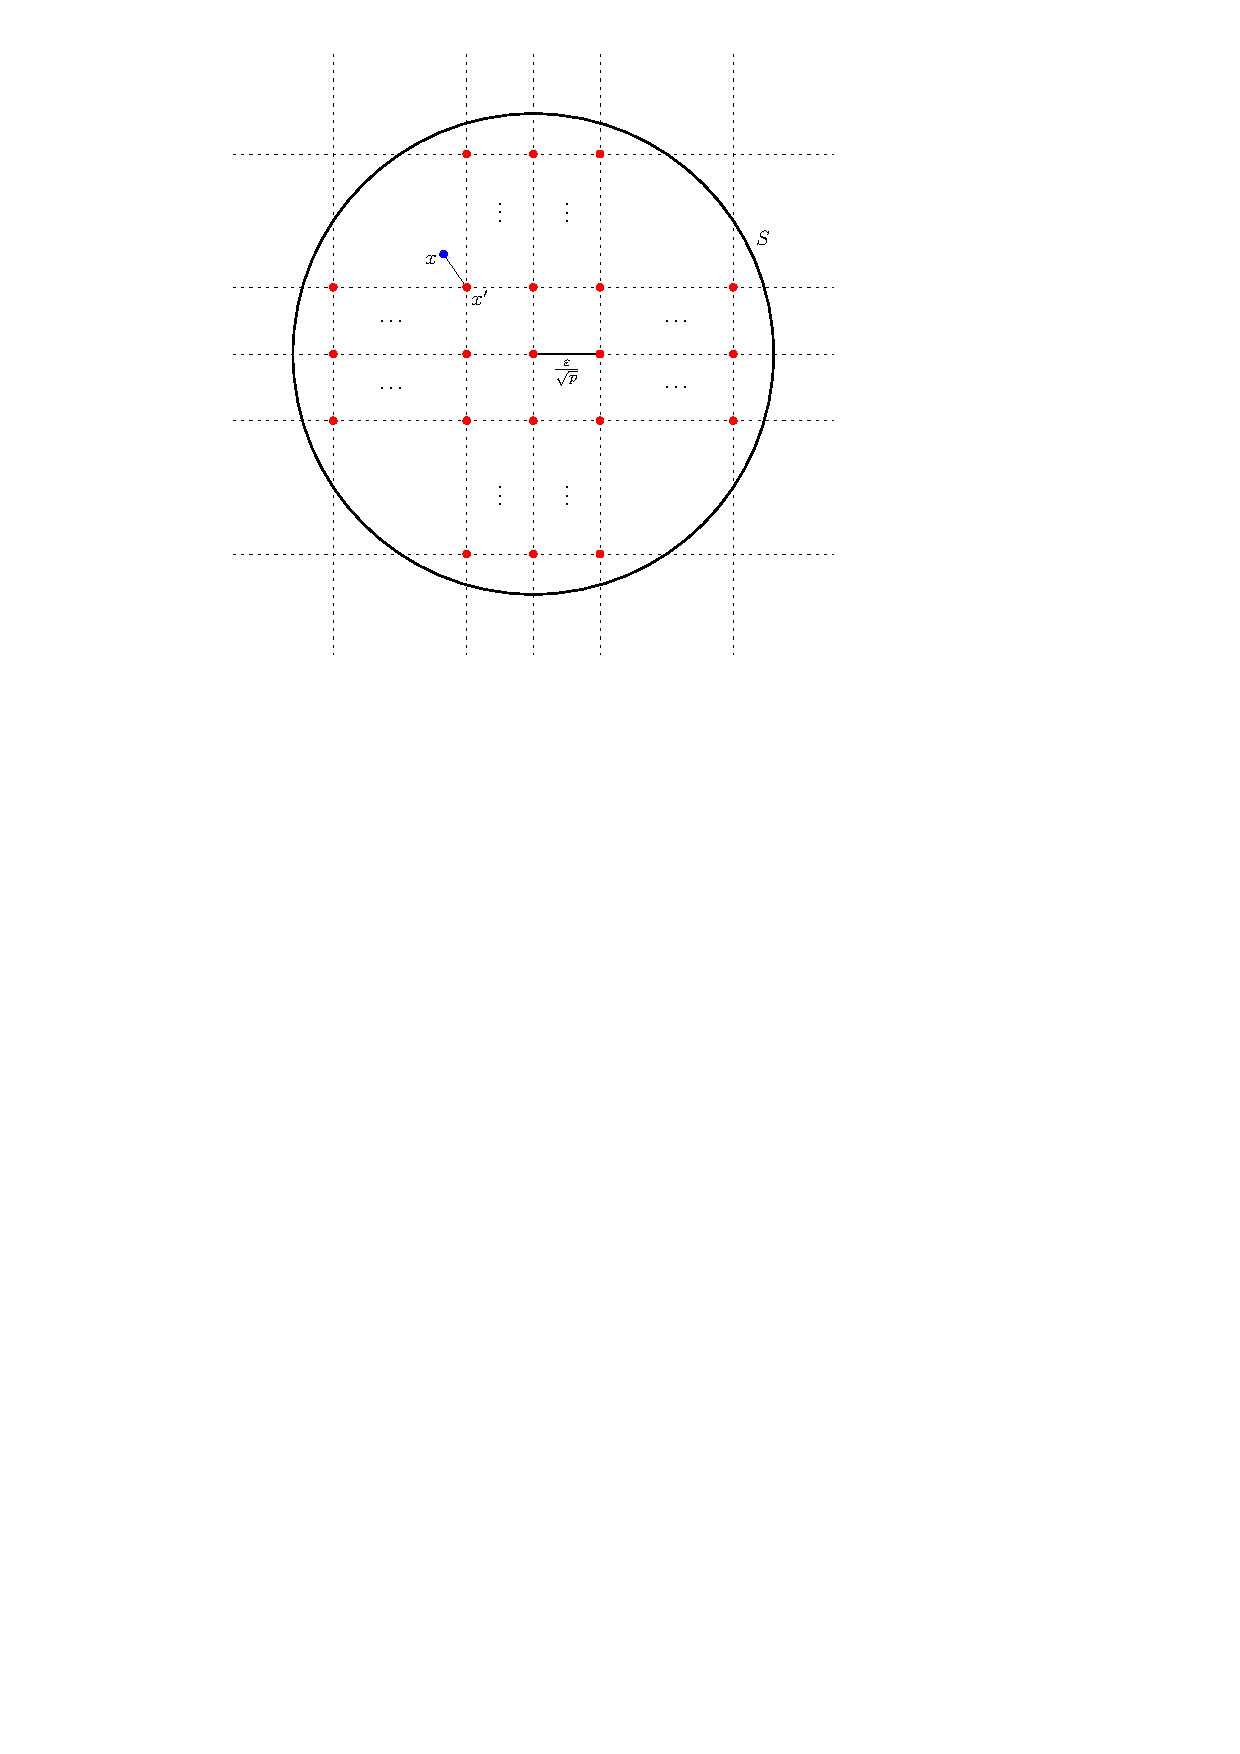
\includegraphics[scale=0.65]{ECover.pdf}$$
\caption{Our chosen $\epsilon$-cover (shown in red) of $S$. For $x \in S$, we choose the grid point $x'$ such that $\norm{x-x'}_2 \le \epsilon$.}
\end{figure}

Notice that $\forall x \in S$, there exists a grid point $x' \in C$ such that $|x_i-x_i'| \le \tfrac{\epsilon}{\sqrt{p}}$ for each $i$. Therefore,
$$\norm{x-x'}_2 = \sqrt{\sum_{i = 1}^p |x_i - x_i'|^2} \leq \sqrt{p\cdot \frac{\epsilon^2}{p}} = \epsilon.$$
This verifies that $C$ is an $\epsilon$-cover of $S$ with respect to the $\ell_2$-norm.

We now bound the size of $C$. Since each $k_i$ in the definition of $C$ has at most $2\tfrac{B\sqrt{p}}{\epsilon}+1$ choices, we have 
$$|C| \le \left( \frac{2B\sqrt{p}}{\epsilon} +1\right)^p \le \left(\frac{3B\sqrt{p}}{\epsilon}\right)^p. \footnote{We assume that $\epsilon \le B \sqrt{p}$. Otherwise, $S$ is contained in the ball centered at the origin with radius $\epsilon$.}$$
\end{proof}




\begin{remark}
In fact, we can prove a stronger version of Lemma \ref{ECSize} that there exists an $\epsilon$-cover of $S$ with at most $\left(\frac{3B}{\epsilon}\right)^p$ elements. We will leave this as a homework exercise.
\end{remark}

\subsubsection{Proof of Theroem \ref{main}}

We are now ready to prove Theorem \ref{main}. 
\begin{proof}[Proof of Theorem \ref{main}]
Let $\delta, \epsilon>0$ be parameters to be specified later. Let $C$ be the $\epsilon$-cover of our parameter space $S$ with respect to the $\ell_2$-norm constructed in Lemma \ref{ECSize}. By part (2) of Theorem 2 from last time, we have
\begin{equation}\label{boundlasttime}
    \forall \theta \in C, |\hat L(\theta) - L(\theta)| \le \delta
\end{equation}
with probability $\ge 1 - 2|C|\exp(-\tfrac{n\delta^2}{2M^2})$. \footnote{Here, we have an additional multiplicative factor of $\frac{1}{4M^2}$ in the exponent, as compared to part (2) of Theorem 2 from last time. The reason is that in our Theorem \ref{main}, the loss function $l((x,y),\theta)$ takes value in the interval $[-M, M]$ (whose width is $2M$), while in Theorem 2 of last time, the range is $[0,1]$. Thus the factor of $\frac{1}{4M^2}$ pops out as we apply Hoeffding's inequality.} We refer to this event as $E$.

Now for any $\theta \in S$, we can pick $\theta_0 \in C$ such that $\norm{\theta-\theta_0}_2 \le \epsilon$. Using the $L$-Lipschitz assumption on the functions $L$ and $\hat L$, we have
$$  |L(\theta) - L(\theta_0)| \le L \norm{\theta-\theta_0}_2 \le L\epsilon,$$
$$  |\hat L(\theta) - \hat L(\theta_0)| \le L \norm{\theta-\theta_0}_2 \le L\epsilon.$$
Therefore, by (\ref{boundlasttime}) conditioned on $E$, we have
\begin{equation} \label{triangle}
    |\hat L(\theta) -  L(\theta)| \le |\hat L(\theta)-\hat L(\theta_0)| + |\hat L(\theta_0) -  L(\theta_0)| + | L(\theta_0) - L(\theta)| \le 2L\epsilon+\delta.
\end{equation}


It remains to choose suitable parameters $\delta$ and $\epsilon$ to get the desired bound in Theorem \ref{main} while making the failure probability small. We set
$$  \delta = 10\sqrt{\frac{M^2p\log(LBn)}{n}}, \text{ and } \epsilon = \frac{\delta}{2L}.$$
In this way, we see from (\ref{triangle}) that
$$  |\hat L(\theta)- L(\theta)| \le 2L\epsilon + \delta = 2\delta \lesssim M\sqrt{\frac{p\log(LBn)}{n}}.$$
Finally, we estimate the failure probability for this choice of $\delta$ and $\epsilon$. We have
\begin{align*}
    |C|\exp\left(-\frac{n\delta^2}{M^2}\right) &\le \left(\frac{3B\sqrt{p}}{\epsilon}\right)^p \exp \left( - \frac{n(100M^2p\log(LBn))}{nM^2} \right)   \\
        &= \exp\left(p\log\left(\frac{6LB\sqrt{p}}{\delta}\right) - 100p\log(LBn) \right)\\
        &= \exp\left(p\log(6LB\sqrt{n}) - p \log(10M\sqrt{\log{LBn}}) - 100p\log(LBn)\right)\\
        &= \exp \left( p\left(-\frac{199}{2}\log n - \frac{1}{2} \log \log n  + \log 6 - \log (10M) -99 \log(LB) - \frac{1}{2} \log \log (LB)   \right) \right)\\
        &\le \exp \left( p\left(\log 6 - \log (10M) -99 \log(LB) - \frac{1}{2} \log \log (LB)   \right) \right)\\
        &\le O(e^{-p}),
\end{align*}
as long as $M, L, B$ are greater than some small constant.
Hence we have actually proven the stronger bound on the failure probability in Remark \ref{Tight}.
\end{proof}


\section{Concentration Inequalities}
In this section, we will look at a few tools for bounding the tail distribution of a random variable. These bounds can be very useful in estimating the failure probability of a certain event of interest. For example, as we saw from the last lecture, we can use Hoeffding's inequality to bound the failure probability of uniform convergence for finite hypothesis classes. Let us recall the statement of Hoeffding's inequality:

\begin{proposition}[Hoeffding's inequality]
Let $X_1, \dots, X_n$ be independent random variables such that $a_i \le X_i \le b_i$ almost surely for each $i \in [n]$. Let
$$  \hat \mu = \sum_{i=1}^n X_i, \mu = \E\left[\sum_{i=1}^n X_i \right].$$
Then for any $t>0$, we have
$$  \Pr[|\hat\mu - \mu| \ge t] \le 2\exp \left( -\frac{2t^2}{\sum_{i=1}^n (b_i-a_i)^2} \right).    $$
\end{proposition}

In order to prove Hoeffding's inequality, we will first look at two other basic concentration inequalities: Markov's inequaility and Chebyshev's inequality. We will then apply these simpler concentration inequalities to the moment generating function of the random variable $\hat \mu$ to obtain a heuristic argument for Hoeffding's inequality. A good reference for our discussion here is Chapter 2 of \cite{W}.


\subsection{Markov's Inequality and Chebyshev's Inequality}

\begin{proposition}[Markov's inequality]
Let $X$ be a non-negative random variable. Then for any $t>0$, we have
$$  \Pr[X \ge t] \le \frac{\E[X]}{t}.   $$
\end{proposition}

\begin{proposition}[Chebyshev's inequality]
Let $Z$ be a random variable. Then for any $t>0$, we have
$$  \Pr[|Z - \E[Z]| \ge t] \le \frac{\Var(Z)}{t^2}. $$
\end{proposition}

Here is a proof of Chebyshev's inequality using Markov's inequality:
\begin{proof}
Note that
$$  \Pr[|Z-\E[Z]| \ge t] = \Pr[|Z-\E[Z]|^2 \ge t^2].    $$
Now applying Markov's inequality to the non-negative random variable $(Z-\E[Z])^2$, we get
$$  \Pr[|Z-\E[Z]|^2 \ge t^2] \le \frac{\E[(Z-\E[Z])^2]}{t^2} = \frac{\Var(Z)}{t^2}.    $$
\end{proof}
In fact, for any positive integer $k$, we have
$$  \Pr[|Z-\E[Z]| \ge t] = \Pr[|Z-\E[Z]|^k \ge t^k].    $$
The same procedure can be applied to non-decreasing functions other than polynomials. For example, for $\lambda \ge 0$, we have
\begin{equation}\label{ExpLambda}
    \Pr[Z-\E[Z] \ge t] = \Pr[e^{\lambda(Z-\E[Z])} \ge e^{\lambda t}] \le \frac{\E[e^{\lambda(Z-\E[Z])}]}{e^{\lambda t}},
\end{equation}
where the last inequality again follows from Markov's inequality.

One may attempt to prove Hoeffding's inequality using Chebyshev's inequality as follows. Assume that $a_i = 0$, $b_i =1$ for each $i$. Let $Z = \hat \mu$. Since $X_1, \ldots, X_n$ are independent, we have 
$$  \Var(Z) = \Var \left(\sum_{i = 1}^n X_i \right) = \sum_{i=1}^n \Var(X_i) \le n.$$
Now Chebyshev's inequality tells us
$$  \Pr[|\hat \mu - \mu| \ge t] \le \frac{\Var(Z)}{t^2} \le \frac{n}{t^2}.  $$
If we set $t = c\sqrt{n}$, then the above becomes
$$  \Pr[|\hat \mu-\mu| \ge c\sqrt{n}] \le \frac{1}{c^2}.    $$
However, Hoeffding's inequality in this case reads as
$$  \Pr[|\hat \mu-\mu| \ge c\sqrt{n}] \le 2e^{-2c^2}.    $$
So this attempt does not give us what we want.


\subsection{Moment Generating Function}
Based on (\ref{ExpLambda}), we may also try to prove Hoeffding's inequality using the moment generating function of our random variable $Z = \hat \mu = \sum_{i=1}^n X_i$. Let us first recall the definition:

\begin{definition}
The \emph{moment generating function} of a random variable $X$, denoted $M_X$, is given by
$$  M_X(\lambda) = \E[e^{\lambda X}]. $$
\end{definition}

Using Taylor expansion, the above definition can be rewritten as
$$  \E[e^{\lambda X}] = \E\left[1 + \lambda X + \frac{(\lambda X)^2}{2!} + \cdots \right] = 1 + \lambda \E[X] + \frac{\lambda^2}{2}\E[X^2] + \cdots. $$
This applied to the random variable $X - \E[X]$ gives
\begin{equation}\label{MomentVar}
    \E[e^{\lambda(X - \E[X])}] = 1 + \lambda \E[X - \E[X]] + \frac{\lambda^2}{2}\E[(X - \E[X])^2] + \cdots = 1 + \lambda^2\Var(X) + \cdots. 
\end{equation}  

Back to our case $Z = \sum_{i=1}^n X_i$. Since $X_1, \dots, X_n$ are independent, we have
$$  \E[e^{\lambda(\Z - \E[Z])}] = \E[e^{\lambda(X_1 - \E[X_1])}\cdots e^{\lambda(X_n - \E[X_n])}] =  \E[e^{\lambda(X_1 - \E[X_1])}] \cdots \E[e^{\lambda(X_n - \E[X_n])}]. $$
Hence by (\ref{ExpLambda}), we have the following bound:
$$  \Pr[Z-\E[Z] \ge t] \le \inf_{\lambda \ge 0} \frac{\E[e^{\lambda(X_1 - \E[X_1])}] \cdots \E[e^{\lambda(X_n - \E[X_n])}]}{e^{\lambda t}}, $$
i.e.,
\begin{equation}\label{LogBound}
    \log \Pr[Z-\E[Z] \ge t] \le \inf_{\lambda \ge 0} \sum_{i = 1}^n \log \E[e^{\lambda(X_1 - \E[X_1])}] - \lambda t.
\end{equation}

Now in the case $X_i \in [0,1]$ for each $i \in [n]$, we give a heuristic argument for Hoeffding's inequality. In this case, $\Var(X_i) \le 1$ for each $i \in [n]$, so from (\ref{MomentVar}) we get
$$  \E[e^{\lambda(X_i - \E[X_i])}] = 1 + \frac{\lambda^2}{2} + \mbox{higher order terms},  $$
for each $i \in [n]$. If we can get rid of these higher order terms in some way, we get
$$  \E[e^{\lambda(X_i - \E[X_i])}] = 1 + \frac{\lambda^2}{2}    $$
for each $i \in [n]$. Thus the right hand side of (\ref{LogBound}) now becomes
$$  \inf_{\lambda \ge 0} \left(n \log \left(1 + \frac{\lambda^2}{2} \right) - \lambda t \right).$$
When $\lambda$ is small, $\log \left(1 + \frac{\lambda^2}{2}\right)$ can be approximated by $\frac{\lambda^2}{2}$. So the above becomes
$$  \inf_{\lambda \ge 0} \frac{n \lambda^2}{2} - \lambda t = -\frac{t^2}{2n}.$$
The ``result" above is not quite the same as Hoeffding's inequality, but has the same magnitude. Hopefully some modification of this argument could give us an actual proof. We will continue the discussion next time.


\bibliography{10_03_final}
\bibliographystyle{plain}
\nocite{*}

%%%%%%%%%%%%%%%%%%%%%%%%%%%%%%%%%%%%%%%%%%%%%%%%%%%%%%%%%%%%%%%%

\end{document}